\documentclass[12pt, a4paper]{article}

% Пакети за српски ћирилични текст
\usepackage[T2A]{fontenc}
\usepackage[utf8]{inputenc}
\usepackage[serbianc]{babel}

% Остали корисни пакети
\usepackage{amsmath}
\usepackage{amssymb}
\usepackage{amsthm}
\usepackage{geometry}
\usepackage{hyperref}
\usepackage{graphicx}
\usepackage{float}
\usepackage{listings}
\usepackage{xcolor}
\usepackage[autostyle]{csquotes}
\usepackage{algorithm}
\usepackage{algpseudocode}
\usepackage{tabularx}
\usepackage{tikz}
\usetikzlibrary{automata, positioning, arrows.meta, shapes.geometric, decorations.pathreplacing, fit}

% TLA+ стил за listings
\lstdefinelanguage{tla}{
    morekeywords={MODULE, EXTENDS, VARIABLES, CONSTANTS, ASSUME,
                  INSTANCE, LOCAL, RECURSIVE,
                  IF, THEN, ELSE, CASE, OTHER,
                  LET, IN,
                  TRUE, FALSE, BOOLEAN, STRING,
                  SUBSET, UNION, DOMAIN, ENABLED, UNCHANGED,
                  Init, Next, Spec},
    sensitive=true,
    morecomment=[l]{\*},
    morecomment=[s]{(*}{*)},
    morestring=[b]",
}

\lstset{
    language=tla,
    basicstyle=\ttfamily\small,
    keywordstyle=\bfseries\color{blue!70!black},
    commentstyle=\itshape\color{gray},
    stringstyle=\color{green!50!black},
    frame=single,
    backgroundcolor=\color{gray!8},
    rulecolor=\color{gray!40},
    numbers=left,
    numberstyle=\tiny\color{gray},
    numbersep=6pt,
    breaklines=true,
    keepspaces=true,
    showstringspaces=false,
}

% Подешавање маргина
\geometry{
    left=2.5cm,
    right=2.5cm,
    top=2.5cm,
    bottom=2.5cm
}

% Дефиниција теорема, лема, итд.
\theoremstyle{plain}
\newtheorem{teorema}{Теорема}[section]
\newtheorem{lema}[teorema]{Лема}
\newtheorem{posledica}[teorema]{Последица}

\theoremstyle{definition}
\newtheorem{definicija}[teorema]{Дефиниција}
\newtheorem{primer}[teorema]{Пример}

\theoremstyle{remark}
\newtheorem*{napomena}{Напомена}

% Наслов документа
\title{\textbf{Формалне методе} \\ (Увод у TLA+)}
\author{Филип Марић \\ Александар Ивановић}
\date{\today}

% -------------------------------------------------------
\begin{document}

\maketitle
\newpage
\tableofcontents
\newpage

\section*{Предговор}
Ова скрипта је настала у оквиру предмета \textbf{Формалне методе - напредни концепти} на докторским студијама
из информатике на Математичком факултету универзитета у Београду. У овом тренутку ово је текст у раној
фази писања и садржи грешке које ће аутори исправљати током рада на скрипти. Идеја је свакако
да и будуће генерације студената раде на њој и обогате садржај. Скрипта се бави језиком \textbf{TLA+}
који служи за проверу дизајна система и који су већ користили и користе највеће светске компаније попут:
Мајкрософта, Амазона, MongoDB, и Cockroach Labs. Идеја је да скрипта омогћи лако
инсталирање тла система и да кроз практичне примере објасни основне концепте, како и самог језика, тако
и кроз примере неке свакодневне програмерске праксе из искуства аутора. Такође желимо да повежемо
и укажемо на везе математике и рачунарства као једне од њених најпрактичнијих грана без набацивања
превише теорије.
\newpage

\section{Увод - Шта је TLA?}
TLA је језик који за писање и провервање спецификација или дизајнирање система.
Када имамо нашу спецификацију тада га можемо користити за
тестирање грешака у дизајну и пре него што почнемо са самом имплементацијом система.
Развијен је од стране Леслија Лампорта, који је такође осмислио језик \LaTeX
што је скраћеница од Лампортов \TeX.
TLA је скраћеница за Temportal Logic of Actions (Темпорале Логике Акција).

\subsection{Инсталација}

Да бисмо почели да пишемо и проверавамо TLA+ спецификације, потребно је инсталирати следеће алате:

\begin{itemize}
    \item \textbf{Java} -- TLA+ алати захтевају Java Runtime Environment (JRE 8 или новији).
    Може се преузети са \url{https://www.java.com}.

    \item \textbf{TLA+ Toolbox} -- званични IDE за TLA+, доступан на
    \url{https://github.com/tlaplus/tlaplus/releases}.
    Садржи TLC model checker и TLAPS (TLA+ Proof System).

    \item \textbf{VS Code додатак (алтернатива)} -- за кориснике Visual Studio Code,
    постоји додатак \texttt{TLA+ by alygin} доступан у VS Code Marketplace-у.
\end{itemize}

\subsubsection{Кораци инсталације (TLA+ Toolbox)}

\begin{enumerate}
    \item Преузети инсталациони пакет са званичне странице за свој оперативни систем.
    \item Покренути инсталацију и пратити упутства.
    \item Покренути Toolbox и креирати нови пројекат: \textit{File > Open Spec > Add New Spec}.
    \item Написати прву спецификацију и покренути TLC model checker.
\end{enumerate}
\subsubsection{Кораци инсталације (VS Code еditor)}
У овим материјалима користићемо VS Code editor (надље само \textbf{вс едитор})
и објаснићемо примере и инсталацију на примеру њега у оперативном систему линукс. Напомињемо да се TLA+ Toolbox
више не одржава, али да се и даље може скинути и користити. Вс едитор је постао
стандард за писање спецификација и TLA се може користити кроз њега као додатак.
Иначе напомињемо да је вс едитор постао популаран едитор за разне програмске језике
управо због модуларности коју пружа богат избор додатака.

Изаберемо иконицу са додацима где се они инсталирају као на слици 1.
\begin{figure}[H]
    \centering
    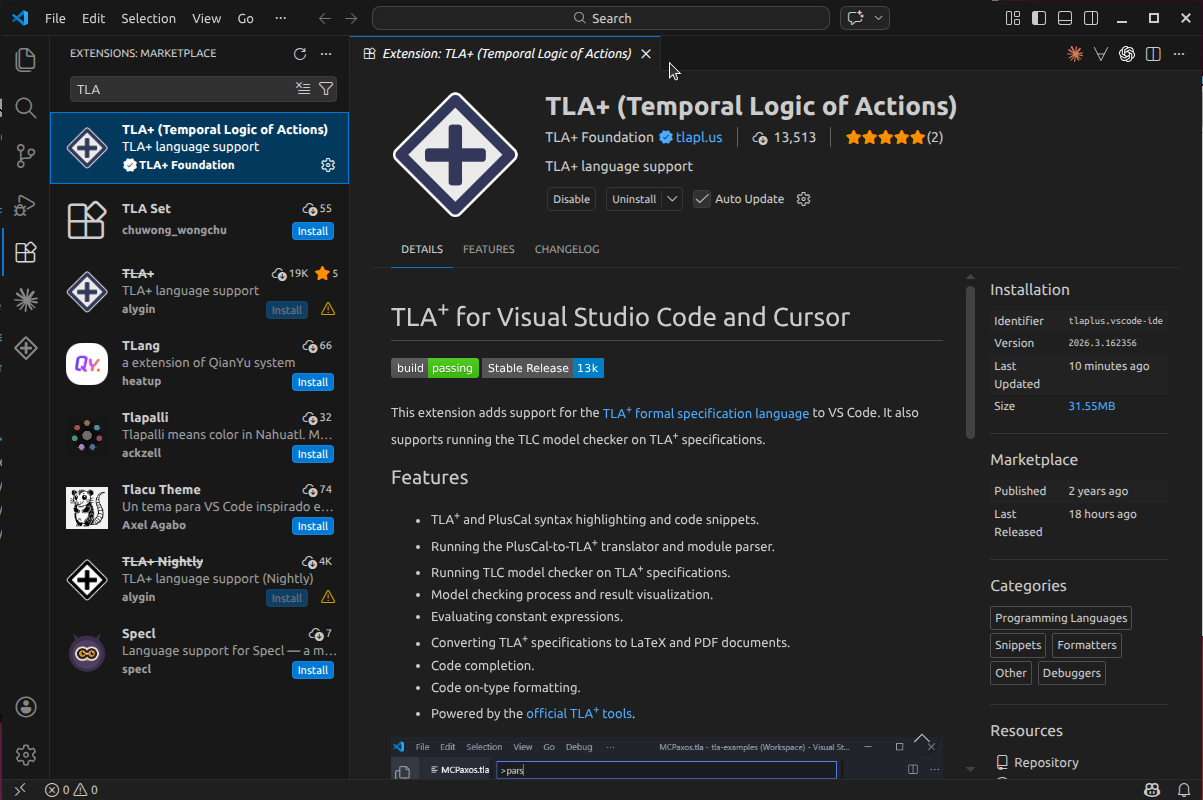
\includegraphics[width=0.7\textwidth]{Images/Instalacija.png}
    \caption{Инсталација TLA+ додатка у VS Code}
\end{figure}
Приликом избора додатка који ћемо инсталирати у претрагу укуцамо
TLA и одаберемо додак као на слици. На крају процеса едитор треба да
изгледа као на слици 2.
\begin{figure}[H]
    \centering
    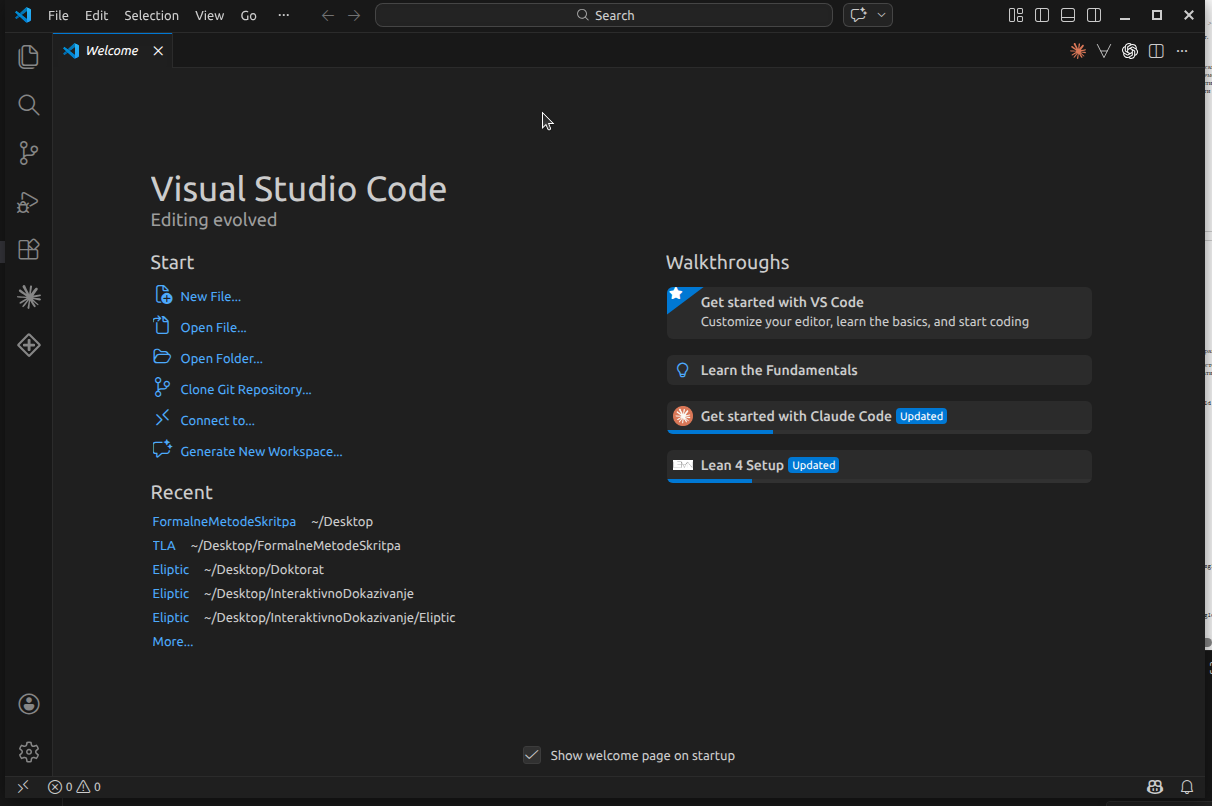
\includegraphics[width=0.7\textwidth]{Images/VSEditor.png}
    \caption{VS Code едитор са TLA+ додатком}
\end{figure}

Сада дајемо мали пример TLA спецификације како би тестирали дали окружење ради добро.

\begin{lstlisting}
---- MODULE Counter ----
EXTENDS Naturals

VARIABLE counter

Init ==
    counter = 1

Next ==
    IF counter < 10
    THEN counter' = counter + 1
    ELSE counter' = counter

Spec ==
    Init /\ [][Next]_counter
====
\end{lstlisting}
У едитору ћемо направити нов текстуални фајл са наставком \textbf{.tla} и
прекопирати претходни код. Пошто смо инсталирали TLA+ додатак на десни клик мишшем
добијамо могућност да одаберемо \textbf{Check model with TLC} као и
 \textbf{Check and debug model with TLC}. \textbf{TLC} је скраћеница за \textbf{TL checker}
и он нам служи да пронађе грешке у нашем дизајну система.
\begin{figure}[H]
    \centering
    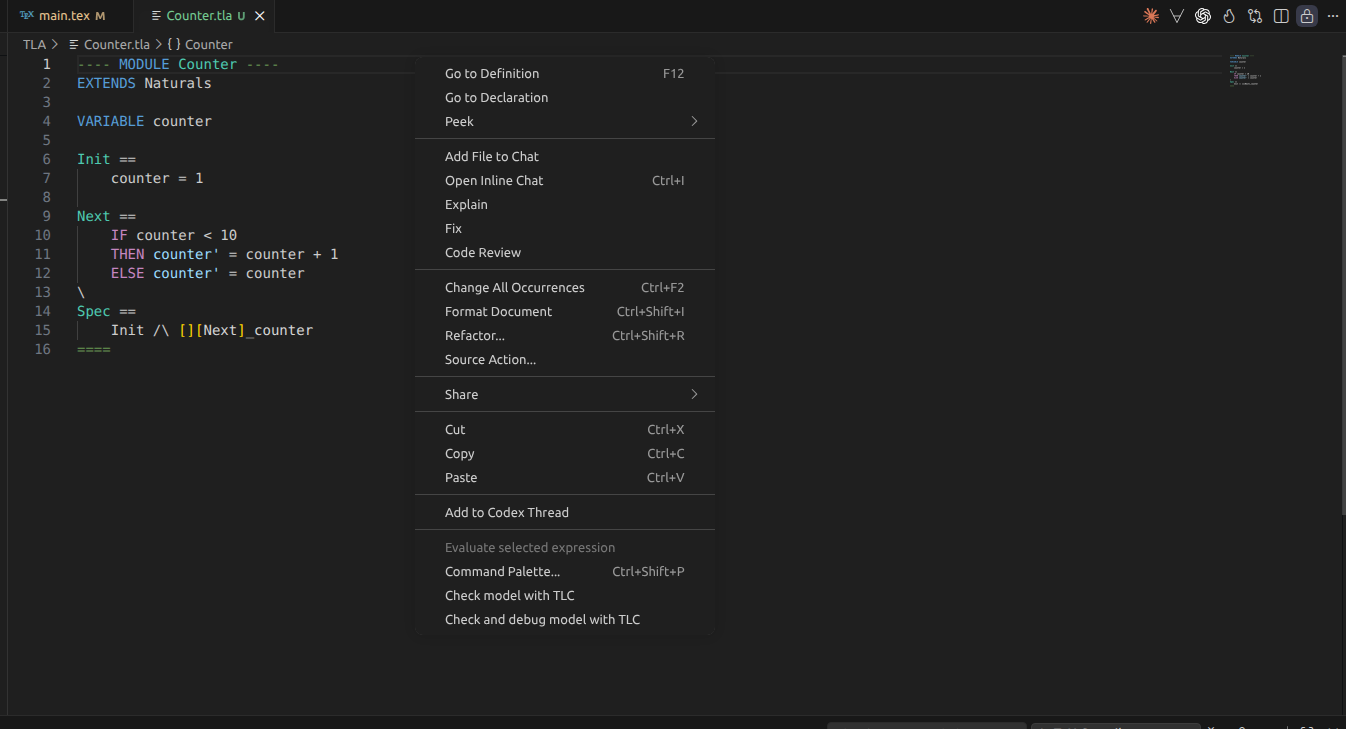
\includegraphics[width=0.7\textwidth]{Images/UvodniPrimer1.png}
    \caption{Код са TLA+ додатком}
\end{figure}
Када кликнемо да проверимо модел тада се може јавити грешака као на следећој слици.
\begin{figure}[H]
    \centering
    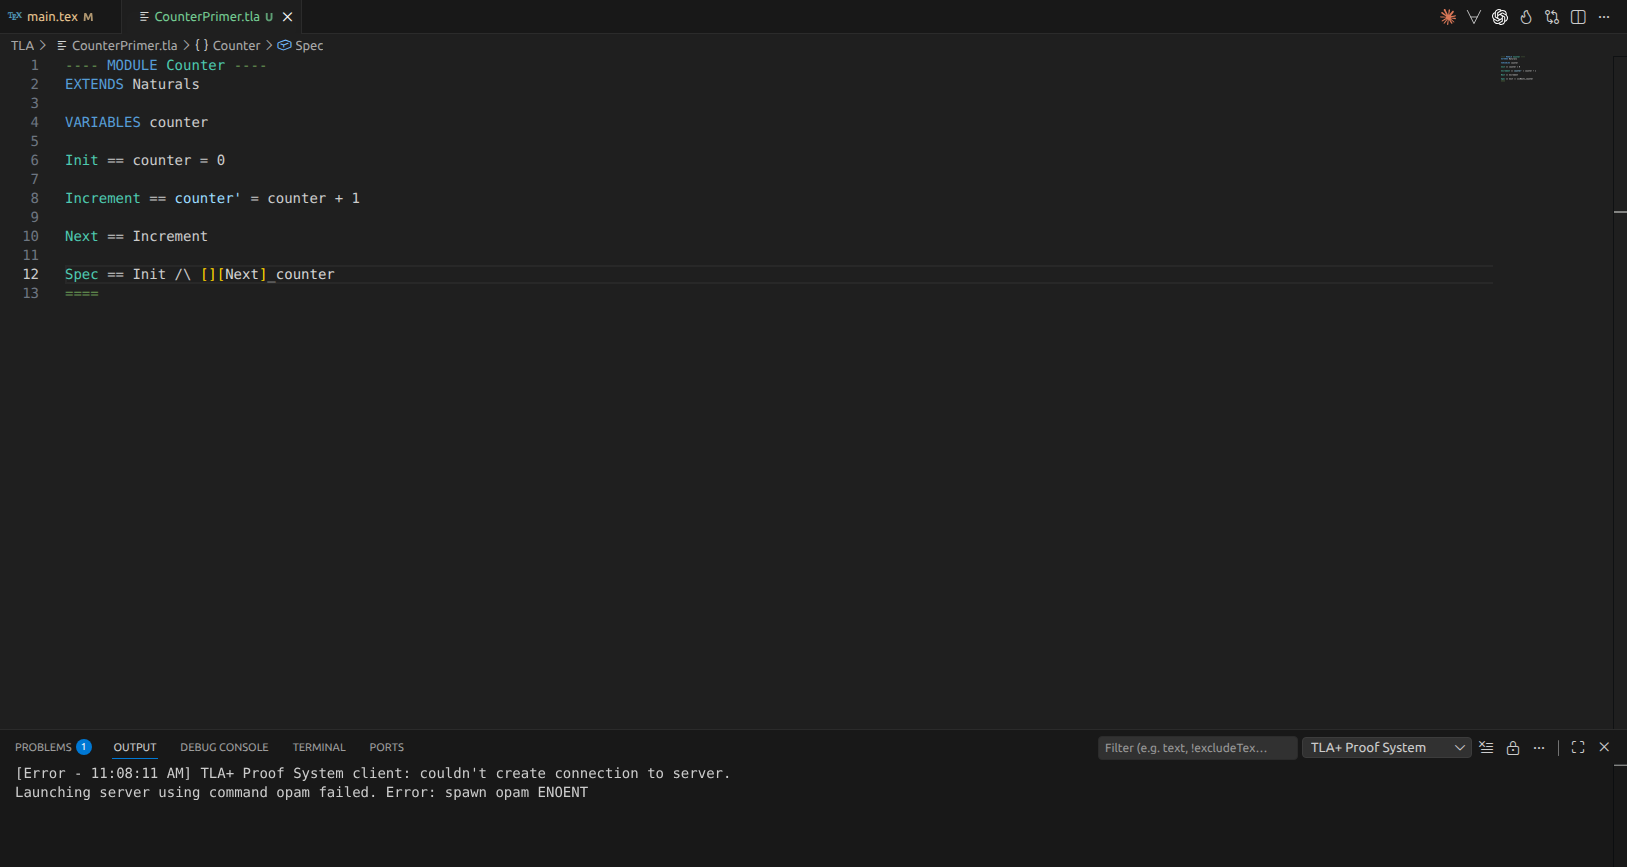
\includegraphics[width=0.7\textwidth]{Images/Greska.png}
    \caption{Грешка при покретању провере}
\end{figure}
Грешка се јавља зато што \textbf{TLAPS - TLA Proof System} покушава да користити
програмски језик \textbf{OCaml}. Ова грешка се на линукс оперативном систему једноставно
решава инсталацијом пакета \textbf{OPAM} следећим командама у терминалу:
\begin{lstlisting}
sudo apt update
sudo apt install opam m4 pkg-config zlib1g-dev gawk time
\end{lstlisting}
Напомињемо да су ово команде за линукс/\textbf{Ubuntu}, ако користите неку другу
дистрибуцију линукса потражите одговарајуће команде.
Уз сваку tla спецификацију (.tla) фајл, такође нам је потребан и конфигурациони
фајл са наставком (.cfg) који нам говори шта су почетна стања, како се прелази у
следеће стање, константе итд.
\begin{lstlisting}
CONSTANTS
    greeting = "Hello"

INIT Init
NEXT Next
\end{lstlisting}
Конфигурациони фајл са претходним кодом морамо да сачувамо у исти фолдер где се налази
и наша спецификација, такође ти фајлови морају имати исто име као и прва линија
у спецификацији (\textbf{Counter.tla}, \textbf{Counter.cfg}).
\begin{lstlisting}
---- MODULE Counter ----
\end{lstlisting}

Кључне ствари које морамо да имамо за сваку спецификацију су:
\begin{enumerate}
    \item Спецификациони фајл са наставком \textbf{.tla}.
    \item Конфигурациони фајл са наставком \textbf{.cfg}.
    \item Они морају да имају исто име, као и име у првој линији у спецификацији.
\end{enumerate}

Пошто смо све урадили, када покренемо проверу спецификације, ако је све у реду
добијамо успех као на слеће две слике.


\begin{figure}[H]
    \centering
    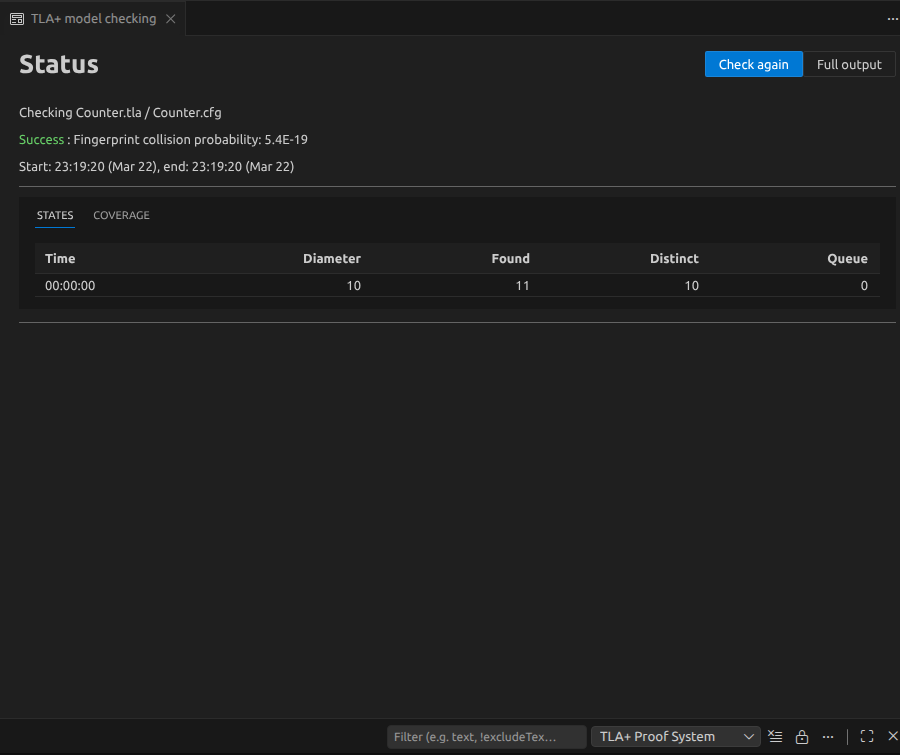
\includegraphics[width=0.7\textwidth]{Images/Uspeh2.png}
    \caption{Успех провера стања}
\end{figure}
\begin{figure}[H]
    \centering
    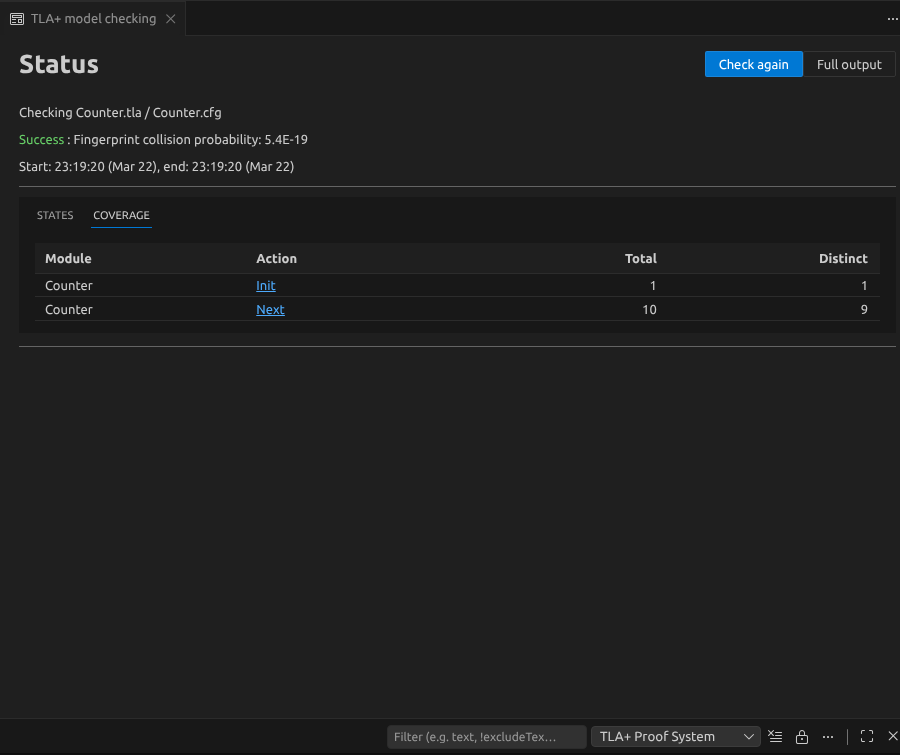
\includegraphics[width=0.7\textwidth]{Images/Uspeh1.png}
    \caption{Успех провера покривености}
\end{figure}
Ово значи да смо успешно успели да инсталирамо tla на линуксу и да наша прва спецификација
система ради без грешке. У следећем поглављу ћемо корак по корак објашњавати шта који део
спецификације значи и чему служи.

\newpage

\section{Основни појмови}
У овом поглављу ћемо да објаснимо основне елементе нашег примера из претходне секције.
Концептуално идеја ТЛА+ је да систем представи као неки граф могућих стања који одређеује
која су почетна, крајња стања и како се прелази у следеће стање система на основу тренутног и правила прелаза.
Ово нас доста подсећа на аутомате из ранијих курсева за комапјлере и лексичку анализу.

\begin{figure}[H]
    \centering
    \begin{tikzpicture}[
        node distance=2.2cm,
        every state/.style={circle, draw, minimum size=1cm},
        ->, >=Stealth, thick,
        lbl/.style={font=\scriptsize, fill=white, inner sep=2pt, align=center}
    ]
        \node[state, initial, initial text={}] (s1)  {$1$};
        \node[state, right=of s1]              (s2)  {$2$};
        \node[state, right=of s2]              (s3)  {$3$};
        \node[right=1.2cm of s3, font=\Large]  (dots){$\cdots$};
        \node[state, right=1.2cm of dots, accepting] (s10) {$10$};

        \draw (s1)   edge node[lbl, above] {$c < 10$\\$c' = c+1$} (s2);
        \draw (s2)   edge node[lbl, above] {$c < 10$\\$c' = c+1$} (s3);
        \draw (s3)   edge node[lbl, above] {$c < 10$\\$c' = c+1$} (dots);
        \draw (dots) edge node[lbl, above] {$c < 10$\\$c' = c+1$} (s10);
        \draw (s10)  edge[loop right] node[lbl, right] {$c \geq 10$\\$c' = c$} (s10);
    \end{tikzpicture}
    \caption{Граф прелаза система Counter: стања су вредности бројача ($c$), прелази одговарају повећавању за 1 све до вредности 10}
\end{figure}
Претходна слика представља граф нашег система  из уводног примера са свим својим могућим стањима. Присећамо се да
почетно стање има само улазну стрелицу, а крајње обележавамо са два концентрична круга. Као што можемо видети почетно стање
нашег система је стање \textbf{1}, а крајње стање је \textbf{10}. Прелаз између стања је могућ ако променљива \textbf{counter}
има вредност мању или једнаку од 10 и ако смо у стањима 1 ди 9. На основу спецификације у тла, тла систем генерише граф стања
система и обилази га и покушава да нађе неке грешке: недоступа стања, бесконачне петље итд.

\subsection{Основни делови tla спецификације}
Да се подсетимо претходног уводног примера и конфигурационог фајла.
\begin{lstlisting}
---- MODULE Counter ----
EXTENDS Naturals

VARIABLE counter

Init ==
    counter = 1

Next ==
    IF counter < 10
    THEN counter' = counter + 1
    ELSE counter' = counter

Spec ==
    Init /\ [][Next]_counter
====
\end{lstlisting}
\begin{lstlisting}
CONSTANTS
    greeting = "Hello"

INIT Init
NEXT Next
\end{lstlisting}
Видимо да уводни пример у потпуности одговара графу који смо нацртали. За велике и озбиљне системе
ручно проверавање стања је практично немогуће и ту нам треба помоћ рачунара. Укратко смо представили
поједностављену верзију како tla систем функционише.
Сваки tla спецификација почиње са кључном речи \textbf{Module}. Симболи \textbf{-\;-\;-}  су део стандардне
синтаксе који означавају име и почетак спецификације. Такође \textbf{=\;=\;=} на самом крају фајла
означава крај спецификације и нема неки већи значај-
\begin{lstlisting}
---- MODULE Counter ----
...
====
\end{lstlisting}

Кључна реч \textbf{EXTENDS Naturals} нам увози библиотеку која нам омогућава да радимо са стандардним аритметичким
операцијама $+, \cdot, >, <$ итд.
\begin{lstlisting}
---- MODULE Counter ----
EXTENDS Naturals
...
====
\end{lstlisting}
Да нисмо увезли ову библиотеку не бисмо могли да радимо са изразима попут $counter < 10$ и $counter + 1$.

\textbf{VARIABLE counter} нам декларише променљиву са именом $counter$.
\begin{lstlisting}
---- MODULE Counter ----
...

VARIABLE counter

Init ==
    counter = 1
...
====
\end{lstlisting}
Променљиве су део стања програма и њихова вредност се мења између стања, тј. при прелазу  између стања
добијају вредности. У нашем случају имамо једну променљиву \texttt{counter} и њена вредност се очигледно
мења при промени стања.
\begin{lstlisting}
Init ==
    counter = 1
\end{lstlisting}
Почетна вреднот променљиве у почетном стању је једнака 1.

Следећи део кода нам говори како се прелази у следеће стање програма и томе служи кључна реч \textbf{Next}.
\begin{lstlisting}
---- MODULE Counter ----
...
Next ==
    IF counter < 10
    THEN counter' = counter + 1
    ELSE counter' = counter
...
====
\end{lstlisting}
Структура \textbf{IF ... THEN ... ELSE} има стандардно значење као и у свим програмским језицима, ако је услов испуњен
улазимо у прву грану, а у супротном у \textbf{ELSE} грану. Оно што се разликује од досадашњег искуства је апостроф
над промљивом \texttt{counter'}. Апостроф овде нам служи да кажемо шта је ново стање променљиве \texttt{counter} и како га добијамо. У овом случају
ново стање променљиве је једнаком старом увећано за 1 ако је вредност из претходног стања мања од 10, а у супротоном
остаје непромењена. Када име променљиве пишемо без апострофа то значи да узимамо њену вредност из претходног стања.

Последњи део спецификације нас асоцира на неки логичку конјукцију два услова. Оператор /\textbackslash\; има 
стандардно значење логичке конјукције $\wedge $, па овај део спецификације можемо тумачити да би спецификација
била исправна потребно је да оба услова буду испуњена.
\begin{lstlisting}
---- MODULE Counter ----
...
Spec ==
    Init /\ [][Next]_counter
====
\end{lstlisting}
Систем је свакако почео у стању \textbf{Init} и вредност променљиве јесте 1 на почетку. Други део конјукције користи
важан оператор \textbf{[]}. Оператор \textbf{[]} значи да неки услов треба да буде испуњен \textbf{увек}, то значи
да има временско трајање, па одатле и добијамо назив TLA - temporal logic of actions. Оператор \textbf{[Next]} нам кажемо
да свако следеће стање при прелазу треба да се добија из стања \textbf{Next}, a \texttt{\_counter} значи да стање може да буде 
непромењено при прелазу. Говорним језиком преведено ова реченица значи да стање почиње из стања \textbf{Init} и прелази могу да се дешавају
само према правилу \textbf{Next} или да стање променљиве \texttt{\_count} остане непромењено. Ако би се десило да у систему
може да се деси неки прелаз који није по правилу tla систем ће да провером да то утврди и пријави грешку.

Потпун преглед оператора се налази у поглављу 4.

\subsection{Конфигурациони фајл}
Конфигурациони фајл има једноставну структуру. У нашем малом примеру дефинише неке константе, дефинише шта је следеће стање
и које је име правила прелаза на следеће могуће знање. 
\begin{lstlisting}
CONSTANTS
    greeting = "Hello"

INIT Init
NEXT Next
\end{lstlisting}
На крају поглавља четири има кратак преглед могућих опција за конфигурациони фајл. 

Упозанавње са осталим могућим операторима и идејама tla спецификације ћемо урадити кроз примере. Треба напоменути
да због специфичности временске компоненте оператора њихова правилна употреба није лака и да је најбоље
упознати се са њима кроз мале практичне примере.

\newpage
\section{Неки основни примери}
Овде дајемо неке примере из рачунарства који су довољно мали али илустративни да се покакжу неки концепти ТЛА
спецификације.

\subsection{Прекидач за светло}
\begin{primer}[Прекидач за светло]
Прекидач за светло је класичан пример коначног аутомата са два стања: \texttt{off} и \texttt{on}.
Једина акција је притискање прекидача (\texttt{Toggle}) која мења стање из \texttt{off} у \texttt{on} и обрнуто.

\textbf{TLA+ модул (\texttt{LightSwitch.tla}):}
\begin{lstlisting}
---- MODULE LightSwitch ----
VARIABLE light

Init == light = "off"

Toggle ==
    \/ /\ light = "off"
       /\ light' = "on"
    \/ /\ light = "on"
       /\ light' = "off"

Next == Toggle

Spec == Init /\ [][Next]_light

TypeInvariant == light \in {"off", "on"}
====
\end{lstlisting}


\textbf{TLC конфигурациони фајл (\texttt{LightSwitch.cfg}):}
\begin{lstlisting}
INIT Init
NEXT Next
INVARIANT TypeInvariant
\end{lstlisting}

Конфигурациони фајл говори TLC model checkeru:
\begin{itemize}
    \item \texttt{INIT} --- која формула описује почетна стања,
    \item \texttt{NEXT} --- која формула описује прелазе стања,
    \item \texttt{INVARIANT} --- које особине треба да важе у \emph{свим} достижним стањима.
\end{itemize}
Овде први пут видимо нови концепт \textbf{INVARIANT} у конфигурационом фајлу. Он нам говори да неки услов
треба да важи у свим стањима наше спецификације и према томе је инваријантан. 
Особина исправности светло је увек у неком од два дозвољена стања, тј. \texttt{TypeInvariant} дефиниција важи у сваком достижном стању.
    
Такође обратимо пажњу на дефиницију 
\begin{lstlisting}
    TypeInvariant == light \in {"off", "on"}
\end{lstlisting}
овде можемо видети такође везу са математиком. Наиме ово је чиста формула теорије скупова која каже променљива \texttt{light}
припада неком скупу могућих вредности. Могли смо записати $x \in \{p, q\}$, идеја програма би имала исти смисао.
\end{primer}

\begin{primer}[Прекидач за светло --- булова варијанта]
Исти прекидач можемо моделовати и са буловом променљивом уместо стрингова.
Вредност \texttt{TRUE} представља укључено светло, \texttt{FALSE} искључено.
Акција \texttt{Toggle} тада постаје знатно краћа јер нема потребе за две гране.

\textbf{TLA+ модул (\texttt{LightSwitchBool.tla}):}
\begin{lstlisting}
---- MODULE LightSwitchBool ----
VARIABLE light

Init == light = FALSE

Toggle == light' = ~light

Next == Toggle

Spec == Init /\ [][Next]_light

TypeInvariant == light \in BOOLEAN
====
\end{lstlisting}

Уочимо неколико ствари. \texttt{Toggle} је сада само \texttt{light' = \textasciitilde light} негација тренутне вредности.
\texttt{TypeInvariant} користи уграђени скуп \texttt{BOOLEAN} $= \{\texttt{TRUE}, \texttt{FALSE}\}$ уместо ручно набројаног скупа стрингова.
Обе варијанте су семантички еквивалентне; булова је компактнија, а стринг варијанта је читљивија када стања имају смислена имена.
\end{primer}

\subsection{Брава на вратима}
\begin{primer}[Брава на вратима]
Брава на вратима је пример са три стања: \texttt{locked}, \texttt{unlocked} и \texttt{open}.
За разлику од прекидача, овде \emph{нису све акције увек дозвољене} нпр.\ врата се не могу отворити ако су закључана.

Акције су:
\begin{itemize}
    \item \texttt{Unlock} --- откључавање (само из стања \texttt{locked}),
    \item \texttt{Lock} --- закључавање (само из стања \texttt{unlocked}),
    \item \texttt{Open} --- отварање (само из стања \texttt{unlocked}),
    \item \texttt{Close} --- затварање (само из стања \texttt{open}).
\end{itemize}

\textbf{TLA+ модул (\texttt{DoorLock.tla}):}
\begin{lstlisting}
---- MODULE DoorLock ----
VARIABLE door

Init == door = "locked"

Unlock == /\ door = "locked"
          /\ door' = "unlocked"

Lock   == /\ door = "unlocked"
          /\ door' = "locked"

Open   == /\ door = "unlocked"
          /\ door' = "open"

Close  == /\ door = "open"
          /\ door' = "unlocked"

Next == Unlock \/ Lock \/ Open \/ Close

Spec == Init /\ [][Next]_door

TypeInvariant == door \in {"locked", "unlocked", "open"}

CannotOpenWhenLocked == door = "locked" => door # "open"
====
\end{lstlisting}

\textbf{TLC конфигурациони фајл (\texttt{DoorLock.cfg}):}
\begin{lstlisting}
INIT Init
NEXT Next
INVARIANT TypeInvariant
INVARIANT CannotOpenWhenLocked
\end{lstlisting}

Кључна разлика у односу на прекидач је да свака акција садржи \textbf{услов изводљивости} (precondition) у првом конјункту.
На пример, \texttt{Open} може да се изврши само ако је \texttt{door = "unlocked"} ако то не важи, акција је блокирана.
TLC ће аутоматски проверити да у ниједном достижном стању \texttt{CannotOpenWhenLocked} не буде нарушена.
\end{primer}

\subsection{Узајамно искључење}
\begin{primer}[Узајамно искључење]
Узајамно искључење (\textit{mutual exclusion}) је класичан проблем у теорији конкурентних система.
Два процеса се такмиче за приступ критичној секцији, делу кода који смем да се извршава само један процес истовремено.
Сваки процес може бити у једном од три стања: \texttt{idle} (не покушава улазак), \texttt{trying} (чека на улазак) и \texttt{critical} (у критичној секцији).

Овај пример је значајан јер уводи два кључна концепта:
\begin{itemize}
    \item моделовање \textbf{вишеструких процеса} --- стање система је функција која сваком процесу додељује његово тренутно стање,
    \item \textbf{safety особина} --- гарантује да два процеса никад нису истовремено у критичној секцији.
\end{itemize}

\textbf{TLA+ модул (\texttt{MutualExclusion.tla}):}
\begin{lstlisting}
---- MODULE MutualExclusion ----
EXTENDS Naturals

CONSTANT N
ASSUME N \in Nat /\ N > 0

Procs == 1..N

VARIABLE state

States == {"idle", "trying", "critical"}

Init == state = [p \in Procs |-> "idle"]

TryEnter(p) ==
    /\ state[p] = "idle"
    /\ state' = [state EXCEPT ![p] = "trying"]

Enter(p) ==
    /\ state[p] = "trying"
    /\ \A q \in Procs : q # p => state[q] # "critical"
    /\ state' = [state EXCEPT ![p] = "critical"]

Exit(p) ==
    /\ state[p] = "critical"
    /\ state' = [state EXCEPT ![p] = "idle"]

Next == \E p \in Procs : TryEnter(p) \/ Enter(p) \/ Exit(p)

Spec == Init /\ [][Next]_state

TypeInvariant == \A p \in Procs : state[p] \in States

MutualExclusion == \A p, q \in Procs : p # q => ~(state[p] = "critical" /\ state[q] = "critical")
====
\end{lstlisting}

\textbf{TLC конфигурациони фајл (\texttt{MutualExclusion.cfg}):}
\begin{lstlisting}
CONSTANTS
    N = 2

INIT Init
NEXT Next
INVARIANT TypeInvariant
INVARIANT MutualExclusion
\end{lstlisting}

Уочимо неколико важних ствари.
Стање система је \textbf{функција} \texttt{state}, дефинисана над скупом процеса \texttt{Procs = 1..N}.
Израз \texttt{state[p]} даје тренутно стање процеса \texttt{p}, а \texttt{[state EXCEPT ![p] = v]} прави нову функцију идентичну \texttt{state} осим за процес \texttt{p}.

Акција \texttt{Enter(p)} садржи услов \texttt{\textbackslash A q \textbackslash in Procs : q \# p => state[q] \# "critical"} --- процес \texttt{p} може ући у критичну секцију само ако ниједан други процес тренутно није у њој.
Ово је сама суштина узајамног искључења директно изражена у спецификацији.

Особина \texttt{MutualExclusion} формално каже: за свака два различита процеса \texttt{p} и \texttt{q}, не може се десити да су оба у стању \texttt{critical} истовремено.
TLC ће ову особину проверити у свим достижним стањима.
\end{primer}


\newpage
\section{Напредни примери}
Ови примери претпостављају познавање основних концепата TLA+ и приказују реалистичније системе
са вишеструким процесима, збиркама порука и нетривијалним особинама исправности.

\subsection{Outbox pattern}
\begin{primer}[Outbox pattern]
Outbox pattern је техника којом се у истој трансакцији уписује промена у базу и порука у \texttt{outbox} табелу.
Засебан процес затим чита \texttt{outbox} и шаље поруке ка брокеру, па се порука чисти тек након потврде.

\textbf{TLA+ код (издвојени део спецификације):}
\begin{lstlisting}
VARIABLES db, outbox, broker, sent, acked, allMsgs, nextMsgId

CreateOrder(o) ==
    LET m == [id |-> nextMsgId, order |-> o] IN
    /\ db[o] = "NEW"
    /\ db' = [db EXCEPT ![o] = "CREATED"]
    /\ outbox' = outbox \cup {m}
    /\ allMsgs' = allMsgs \cup {m}
    /\ nextMsgId' = nextMsgId + 1
    /\ UNCHANGED <<broker, sent, acked>>

RelaySend(m) ==
    /\ m \in outbox
    /\ broker' = broker \cup {m}
    /\ sent' = sent \cup {m.id}
    /\ UNCHANGED <<db, outbox, acked, allMsgs, nextMsgId>>

AckFromBroker(m) ==
    /\ m \in broker
    /\ acked' = acked \cup {m.id}
    /\ UNCHANGED <<db, outbox, broker, sent, allMsgs, nextMsgId>>

CleanupOutbox(m) ==
    /\ m \in outbox
    /\ m.id \in acked
    /\ outbox' = outbox \ {m}
    /\ UNCHANGED <<db, broker, sent, acked, allMsgs, nextMsgId>>
\end{lstlisting}
\end{primer}
\newpage
\section{Доказивање теорема у TLA+}

TLA+ не служи само за проверу модела \textit{(model checking)} тј. TLC проверава особине прегледом свих достижних стања,
што је изводљиво само за коначне моделе са конкретним вредностима константи.
За бесконачне системе или потпуно опште доказе користи се \textbf{TLAPS} (\textit{TLA+ Proof System}),
алат за формалне дедуктивне доказе директно у TLA+ синтакси \cite{tlapsProofTactics}.

TLAPS преводи доказе теорема на позадинске доказиваче теорема:
\begin{itemize}
    \item \textbf{Zenon} је аутоматски доказивач за логику првог реда,
    \item \textbf{Isabelle/TLA+} је интерактивни доказивач теорема,
    \item \textbf{SMT решавачи} нпр.\ Z3 за аритметичке леме.
\end{itemize}

\subsection{Инсталација TLAPS}
TLAPS долази као посебна инсталација и није део додатка за VS Code едитор. Потребно га је скинути
са званичног GitHub репозиторијума
\url{https://github.com/tlaplus/tlapm}. Када се скине инсталациони фајл, тада се .bin фајл за инсталацију
може локално инсталирати на следећи начин на десктопу
\begin{lstlisting}[language=bash]
./tlaps-*.bin -d $HOME/Desktop/tlaps
\end{lstlisting}
Када се заврши инсталација TLAPS можемо додати путању ка bin фолдеру како бисмо из тренутне сесије
терминала могли да покрећемо tlapm.
\begin{lstlisting}[language=bash]
export PATH=$PATH:~/Desktop/tlaps/bin
\end{lstlisting}
Да би проверили да ли TLAPS систем ради можемо покренути команду
\begin{lstlisting}[language=bash]
tlapm --version
\end{lstlisting}
Ако се појави број верзије система то значи да смо успешно инсталирали програм.
Напомињемо овде да је овде показана локална инсталација јер лако омогућава да се програм обрише без икаквих
системских измена. Ако се прекине тренутна сесија терминала морамо опет команду export, на тај начин
не дирамо системске путање. Овај приступ је одабран јер је релативно лаган да се уради без икакве шансе да се 
направи неки проблем. 

Могуће је повезати TLAPS са VS Code едитором и Toolbox-ом и покретати га тако или на начин који смо описали из терминала.

Када све ради како треба и када имамо нашу спецификацију са доказом неке теореме тада покренемо tlapm 
\begin{lstlisting}[language=bash]
tlapm <ime>.tla
\end{lstlisting}
излаз који добијамо у терминлу
\begin{lstlisting}[language=bash]
aleksandar@aleksandar-A520M-K-V2:~/Desktop/FormalneMetodeSkritpa/TLA$ tlapm LightSwitchProof.tla 
(* created new ".tlacache/TLAPS.tlaps/TLAPS.thy" *)
(* fingerprints written in ".tlacache/TLAPS.tlaps/fingerprints" *)
File "/home/aleksandar/Desktop/TLAPS/lib/tlaps/TLAPS.tla", line 1, character 1 to line 362, character 77:
[INFO]: All 0 obligation proved.
** Unexpanded symbols: ---

** Unexpanded symbols: STATE_TypeInvariant_, ACTION_Toggle_

** Unexpanded symbols: ---

** Unexpanded symbols: ---

(* created new ".tlacache/LightSwitchProof.tlaps/LightSwitchProof.thy" *)
(* fingerprints written in ".tlacache/LightSwitchProof.tlaps/fingerprints" *)
File "./LightSwitchProof.tla", line 1, character 1 to line 32, character 4:
[INFO]: All 12 obligations proved.
\end{lstlisting}
где нам на самом крају пише да су све обавезе доказане. Такође се генеришу и неки додатни фајлови са Isabelle доказом,
као што се може видети из порука са терминала.
\subsection{Структура доказа}

Доказ у TLA+ је \textbf{хијерархијски}. Разлаже се на нивое означене угластим заградама
\texttt{<1>}, \texttt{<2>}, \texttt{<3>} итд.\ Сваки корак се означава бројем, нпр.\ \texttt{<1>1}, \texttt{<1>2}.

Кључне конструкције:

\begin{center}
\begin{tabularx}{\textwidth}{|l|X|}
\hline
\textbf{Конструкција} & \textbf{Значење} \\
\hline
\texttt{THEOREM P} & исказ теореме коју треба доказати \\
\texttt{ASSUME H PROVE P} & доказ под претпоставком \texttt{H} \\
\texttt{BY facts} & закључи корак из наведених чињеница \\
\texttt{BY DEF Ime} & закључи разматрањем дефиниције \texttt{Ime} \\
\texttt{<1>n. QED} & завршни корак нивоа, обједињује претходне кораке у доказ\\
\texttt{PTL} & позива позадински доказивач за темпоралну логику \\
\hline
\end{tabularx}
\end{center}

\subsection{Пример: бројач са инваријантом}

Моделујемо бројач који почиње од нуле и увећава се за један у сваком кораку.
Желимо да формално докажемо да вредност бројача увек остаје природан број.
То је особина која важи за \emph{све} вредности бројача, без обзира на величину.

\begin{primer}[Доказ инваријанте бројача]

\textbf{TLA+ модул (\texttt{CounterProof.tla}):}
\begin{lstlisting}
---- MODULE CounterProof ----
EXTENDS Naturals, TLAPS

VARIABLE x

Init == x = 0
Next == x' = x + 1
Spec == Init /\ [][Next]_x

Inv == x \in Nat

THEOREM Spec => []Inv
<1>1. Init => Inv
      BY DEF Init, Inv
<1>2. Inv /\ [Next]_x => Inv'
      BY DEF Inv, Next
<1>3. QED
      BY <1>1, <1>2, PTL DEF Spec
====
\end{lstlisting}

Теорема каже: ако систем задовољава спецификацију \texttt{Spec}, онда \texttt{Inv} важи у
\emph{свим} стањима (темпорална формула \texttt{[]Inv}).

Доказ се одвија у три корака на нивоу \texttt{<1>}:
\begin{itemize}
    \item \texttt{<1>1} --- \textbf{базни случај}: ако је \texttt{Init} тачно, онда је \texttt{Inv} тачно.
    Разматрањем дефиниција: \texttt{Init} каже да је \texttt{x = 0}, а \texttt{Inv} каже да је \texttt{x \textbackslash in Nat} --- пошто је $0 \in \mathbb{N}$, следи тривијално.

    \item \texttt{<1>2} --- \textbf{индуктивни корак}: ако \texttt{Inv} важи у тренутном стању и
    систем изврши корак \texttt{[Next]\_x}, онда \texttt{Inv'} важи у следећем стању.
    Ако је \texttt{x \textbackslash in Nat} и \texttt{x' = x + 1}, онда је \texttt{x' \textbackslash in Nat} јер је скуп природних бројева затворен за сабирање.

    \item \texttt{<1>3. QED} --- обједињује \texttt{<1>1} и \texttt{<1>2} позивањем \texttt{PTL}
    (\textit{Propositional Temporal Logic}) доказивача, који из базног и индуктивног случаја аутоматски изводи \texttt{[]Inv}.
\end{itemize}

Ово је образац \textbf{индуктивне инваријанте}, најчешћа техника доказивања safety особина у TLA+:
\begin{enumerate}
    \item Докажи да инваријанта важи у почетном стању (\textit{база индукције}).
    \item Докажи да ако инваријанта важи пре прелаза, важи и после (\textit{индуктивни корак}).
    \item Из ова два корака TLAPS аутоматски изводи да инваријанта важи увек.
\end{enumerate}
Приметимо из овог примера да ово нисмо могли да докажемо провером модела. Променљива \texttt{x} је типа 
природних бројева и број стања је бесконачан и проверавач модела би се вртео заувек покушавајући да досегне 
и провери сва стања. У оваком слуачју морамо да посегнемо за напреднијим техникама и да формулишемо оваква
тврђења као теореме.
\end{primer}

\begin{primer}[Доказ безбедности прекидача за светло]
Враћамо се на пример прекидача за светло и формално доказујемо да \texttt{light} увек остаје
у скупу дозвољених вредности. Ово је особина коју смо раније само проверавали TLC-ом.

\textbf{TLA+ модул (\texttt{LightSwitchProof.tla}):}
\begin{lstlisting}
---- MODULE LightSwitchProof ----
EXTENDS TLAPS

VARIABLE light

Init == light = "off"

Toggle ==
    \/ /\ light = "off" /\ light' = "on"
    \/ /\ light = "on"  /\ light' = "off"

Next == Toggle

Spec == Init /\ [][Next]_light

TypeInvariant == light \in {"off", "on"}

THEOREM Spec => []TypeInvariant
<1>1. Init => TypeInvariant
      BY DEF Init, TypeInvariant
<1>2. TypeInvariant /\ [Next]_light => TypeInvariant'
  <2>1. ASSUME TypeInvariant, Toggle
        PROVE  TypeInvariant'
        BY <2>1 DEF TypeInvariant, Toggle
  <2>2. ASSUME TypeInvariant, UNCHANGED light
        PROVE  TypeInvariant'
        BY <2>2 DEF TypeInvariant
  <2>3. QED
        BY <2>1, <2>2 DEF Next
<1>3. QED
      BY <1>1, <1>2, PTL DEF Spec
====
\end{lstlisting}

Доказ следи исти образац индуктивне инваријанте, али са мање корака јер систем има само једну акцију.

\begin{itemize}
    \item \texttt{<1>1} у почетном стању \texttt{light = "off"}, па \texttt{light \textbackslash in \{"off", "on"\}} тривијално важи.
    \item \texttt{<1>2}  индуктивни корак се рашчлањује на два подслучаја:
    \begin{itemize}
        \item \texttt{<2>1}: акција \texttt{Toggle} мења \texttt{light} из \texttt{"off"} у \texttt{"on"} или обрнуто, у оба случаја вредност остаје у \texttt{\{"off", "on"\}},
        \item \texttt{<2>2}: ако \texttt{light} остаје непромењено, инваријанта тривијално важи.
    \end{itemize}
    \item \texttt{<1>3. QED}  \texttt{PTL} обједињује базни и индуктивни случај у \texttt{[]TypeInvariant}.
\end{itemize}
\end{primer}


Треба напоменути да провера модела (TLC) и доказивање теорема (TLAPS) се \textbf{допуњују}: TLC је бржи и аутоматски
проналази грешке у конкретним моделима, док TLAPS даје потпун доказ за све могуће вредности параметара.
Уобичајен ток корака је прво верификовати спецификацију са TLC-ом, а затим формално доказати кључне особине са TLAPS-ом.


\newpage
\section{Преглед TLA+ оператора}

У овом поглављу дајемо кратак преглед свих основних TLA+ оператора и кључних речи.

\subsection{Логички оператори}
\begin{center}
\begin{tabularx}{\textwidth}{|c|X|}
\hline
\textbf{Оператор} & \textbf{Опис} \\
\hline
\texttt{/\textbackslash} & Логичко И (\textit{and}) \\
\texttt{\textbackslash/} & Логичко ИЛИ (\textit{or}) \\
\texttt{\textasciitilde} & Логичка негација (\textit{not}) \\
\texttt{=>}             & Импликација: $A \Rightarrow B$ \\
\texttt{<=>}            & Еквиваленција: $A \Leftrightarrow B$ \\
\hline
\end{tabularx}
\end{center}

\subsection{Релацијски и аритметички оператори}
\begin{center}
\begin{tabularx}{\textwidth}{|c|X|}
\hline
\textbf{Оператор} & \textbf{Опис} \\
\hline
\texttt{=}   & Једнакост \\
\texttt{/=}  & Неједнакост \\
\texttt{<}, \texttt{>}, \texttt{<=}, \texttt{>=} & Поређење бројева \\
\texttt{+}, \texttt{-}, \texttt{*}, \texttt{\textbackslash div}, \texttt{\%} & Аритметичке операције (захтева \texttt{EXTENDS Naturals/Integers/Reals}) \\
\hline
\end{tabularx}
\end{center}

\subsection{Оператори стања и прелаза}
\begin{center}
\begin{tabularx}{\textwidth}{|c|X|}
\hline
\textbf{Оператор} & \textbf{Опис} \\
\hline
\texttt{x'}              & Вредност променљиве $x$ у \textbf{следећем} стању \\
\texttt{UNCHANGED x}     & Променљива $x$ не мења вредност: $x' = x$ \\
\texttt{UNCHANGED <<x,y>>} & Ниједна од наведених променљивих се не мења \\
\texttt{[][A]\_x}        & Темпорална формула: $A$ важи у свим прелазима или $x$ остаје непромењено \\
\texttt{<>P}             & Темпорална формула: $P$ ће \textbf{евентуално} постати тачно \\
\texttt{[]P}             & Темпорална формула: $P$ је \textbf{увек} тачно \\
\hline
\end{tabularx}
\end{center}

\subsection{Теоријско-скуповни оператори}
\begin{center}
\begin{tabularx}{\textwidth}{|c|X|}
\hline
\textbf{Оператор} & \textbf{Опис} \\
\hline
\texttt{\textbackslash in}    & Припадност скупу: $x \in S$ \\
\texttt{\textbackslash notin} & Неприпадност скупу: $x \notin S$ \\
\texttt{\textbackslash cup}   & Унија скупова: $A \cup B$ \\
\texttt{\textbackslash cap}   & Пресек скупова: $A \cap B$ \\
\texttt{\textbackslash}       & Разлика скупова: $A \setminus B$ \\
\texttt{SUBSET S}             & Скуп свих подскупова скупа $S$ \\
\texttt{UNION S}              & Унија свих елемената скупа скупова $S$ \\
\hline
\end{tabularx}
\end{center}

\subsection{Оператори над функцијама и торкама}
\begin{center}
\begin{tabularx}{\textwidth}{|c|X|}
\hline
\textbf{Оператор} & \textbf{Опис} \\
\hline
\texttt{f[x]}                        & Примена функције $f$ на аргумент $x$ \\
\texttt{[x \textbackslash in S |-> e]} & Дефиниција функције: свако $x$ из $S$ се слика у $e$ \\
\texttt{EXCEPT}                      & Ажурирање функције: \texttt{[f EXCEPT ![x] = v]} \\
\texttt{DOMAIN f}                    & Домен функције $f$ \\
\texttt{<<a, b, c>>}                 & Торка са елементима $a$, $b$, $c$ \\
\hline
\end{tabularx}
\end{center}

\subsection{Квантификатори и \texttt{LET/IN}}
\begin{center}
\begin{tabularx}{\textwidth}{|c|X|}
\hline
\textbf{Оператор} & \textbf{Опис} \\
\hline
\texttt{\textbackslash A x \textbackslash in S : P} & Универзална квантификација: $P$ важи за све $x \in S$ \\
\texttt{\textbackslash E x \textbackslash in S : P} & Егзистенцијална квантификација: постоји $x \in S$ за које важи $P$ \\
\texttt{LET x == e IN ...}           & Локална дефиниција: уводи $x$ као скраћеницу за израз $e$ \\
\hline
\end{tabularx}
\end{center}

\subsection{Кључне речи модула}
\begin{center}
\begin{tabularx}{\textwidth}{|c|X|}
\hline
\textbf{Кључна реч} & \textbf{Опис} \\
\hline
\texttt{MODULE}     & Почетак модула \\
\texttt{EXTENDS}    & Увоз другог модула (нпр.\ \texttt{Naturals}, \texttt{Sequences}, \texttt{TLC}) \\
\texttt{CONSTANTS}  & Декларација константи чије вредности се задају у конфигурационом фајлу \\
\texttt{VARIABLES}  & Декларација променљивих стања \\
\texttt{ASSUME}     & Претпоставка о вредности константи \\
\texttt{INSTANCE}   & Инстанцирање другог модула \\
\texttt{Init}       & Предикат почетног стања \\
\texttt{Next}       & Предикат прелаза (дефинише следеће стање) \\
\texttt{Spec}       & Потпуна спецификација система \\
\hline
\end{tabularx}
\end{center}

\subsection{Оператор опсега}
Оператор \texttt{a..b} (из модула \texttt{Naturals} или \texttt{Integers}) прави скуп свих целих бројева од $a$ до $b$ укључујући крајеве.
\begin{center}
\begin{tabularx}{\textwidth}{|c|X|}
\hline
\textbf{Израз} & \textbf{Опис} \\
\hline
\texttt{a..b} & Скуп $\{a, a+1, \ldots, b\}$, нпр.\ \texttt{1..10} даје $\{1,2,\ldots,10\}$ \\
\hline
\end{tabularx}
\end{center}

\subsection{Записи}
Записи (\textit{records}) су структуре са именованим пољима, слично структурама у C-у или речницима у Python-у.
\begin{center}
\begin{tabularx}{\textwidth}{|l|X|}
\hline
\textbf{Синтакса} & \textbf{Опис} \\
\hline
\texttt{[f1 |-> v1, f2 |-> v2]} & Прављење записа са пољима \texttt{f1} и \texttt{f2} \\
\texttt{r.field}                & Приступ пољу \texttt{field} записа \texttt{r} \\
\texttt{[f1 : S1, f2 : S2]}     & Скуп свих записа где \texttt{f1} $\in$ \texttt{S1} и \texttt{f2} $\in$ \texttt{S2} \\
\texttt{[r EXCEPT !.field = v]} & Нови запис идентичан \texttt{r} осим поља \texttt{field} које добија вредност \texttt{v} \\
\hline
\end{tabularx}
\end{center}

\subsection{Секвенце (\texttt{EXTENDS Sequences})}
Секвенце су уређене листе вредности. Да би се користиле потребно је увести модул \texttt{Sequences}.
\begin{center}
\begin{tabularx}{\textwidth}{|l|X|}
\hline
\textbf{Оператор} & \textbf{Опис} \\
\hline
\texttt{<<a, b, c>>}      & Литерал секвенце са елементима $a$, $b$, $c$ \\
\texttt{Len(s)}           & Дужина секвенце \texttt{s} \\
\texttt{Head(s)}          & Први елемент секвенце \texttt{s} \\
\texttt{Tail(s)}          & Секвенца без првог елемента \\
\texttt{Append(s, e)}     & Нова секвенца са елементом \texttt{e} додатим на крај \\
\texttt{s \textbackslash o t} & Конкатенација секвенци \texttt{s} и \texttt{t} \\
\texttt{SubSeq(s, i, j)}  & Подсеквенца од индекса \texttt{i} до \texttt{j} \\
\texttt{s[i]}             & Елемент секвенце на позицији \texttt{i} (индексирање од 1) \\
\hline
\end{tabularx}
\end{center}

\subsection{Оператор \texttt{CHOOSE}}
\texttt{CHOOSE} бира један одређени елемент скупа који задовољава дати предикат.
Важно је напоменути да \texttt{CHOOSE} није случајан избор, увек враћа исти елемент за исти скуп и предикат.
Ако ниједан елемент не задовољава предикат, резултат је недефинисан.
\begin{center}
\begin{tabularx}{\textwidth}{|l|X|}
\hline
\textbf{Синтакса} & \textbf{Опис} \\
\hline
\texttt{CHOOSE x \textbackslash in S : P(x)} & Бира елемент $x$ из скупа $S$ такав да важи $P(x)$ \\
\texttt{CHOOSE x : P(x)}                     & Бира елемент (произвољног типа) такав да важи $P(x)$ \\
\hline
\end{tabularx}
\end{center}

\subsection{Израз \texttt{CASE}}
\texttt{CASE} је условна конструкција са вишеструким гранањем, алтернатива угнежђеним \texttt{IF/THEN/ELSE} изразима.
Грана \texttt{OTHER} покрива све случајеве које претходне гране нису покриле.
\begin{center}
\begin{tabularx}{\textwidth}{|l|X|}
\hline
\textbf{Синтакса} & \textbf{Опис} \\
\hline
\texttt{CASE p1 -> e1}          & Ако је услов \texttt{p1} тачан, вредност је \texttt{e1} \\
\texttt{[] p2 -> e2}            & Ако је услов \texttt{p2} тачан, вредност је \texttt{e2} \\
\texttt{[] OTHER -> e}          & Подразумевана грана ако ниједан услов није тачан \\
\hline
\end{tabularx}
\end{center}

\subsection{Оператори правичности (Fairness)}
Оператори правичности служе за описивање \textit{liveness} особина, гарантују да систем неће заувек
избегавати неку акцију ако је она изводљива.
\begin{center}
\begin{tabularx}{\textwidth}{|l|X|}
\hline
\textbf{Оператор} & \textbf{Опис} \\
\hline
\texttt{WF\_vars(A)} & \textbf{Слаба правичност} (\textit{Weak Fairness}): ако акција $A$ постане трајно изводљива, мора се извршити \\
\texttt{SF\_vars(A)} & \textbf{Јака правичност} (\textit{Strong Fairness}): ако акција $A$ постаје изводљива бесконачно пута, мора се извршити \\
\hline
\end{tabularx}
\end{center}
Слаба правичност спречава да систем „заглави" у стању у ком акција никада није извршена иако је увек могућа.
Јака правичност је строжа, акција се мора извршити чак и ако се изводљивост повремено губи.

\subsection{Оператор \texttt{ENABLED}}
\texttt{ENABLED A} је предикат који је тачан ако и само ако постоји следеће стање у које се може прећи акцијом $A$ из тренутног стања.
\begin{center}
\begin{tabularx}{\textwidth}{|l|X|}
\hline
\textbf{Синтакса} & \textbf{Опис} \\
\hline
\texttt{ENABLED A} & Тачно ако акција $A$ може да се изврши у тренутном стању \\
\hline
\end{tabularx}
\end{center}

\subsection{Модул \texttt{FinSets} (коначни скупови)}
Модул \texttt{FinSets} пружа операторе за рад са коначним скуповима. Увози се са \texttt{EXTENDS FinSets}.
\begin{center}
\begin{tabularx}{\textwidth}{|l|X|}
\hline
\textbf{Оператор} & \textbf{Опис} \\
\hline
\texttt{IsFiniteSet(S)} & Тачно ако је скуп $S$ коначан \\
\texttt{Cardinality(S)} & Број елемената коначног скупа $S$ \\
\hline
\end{tabularx}
\end{center}

\subsection{Конфигурациони фајл (\texttt{.cfg})}
Конфигурациони фајл говори TLC верификатору шта да провери и које вредности да додели константама.
Сваки пројекат има засебан \texttt{.cfg} фајл са истим именом као и модул (нпр.\ \texttt{Counter.cfg}).
\begin{center}
\begin{tabularx}{\textwidth}{|l|l|X|}
\hline
\textbf{Кључна реч} & \textbf{Синтакса} & \textbf{Опис} \\
\hline
\texttt{INIT}              & \texttt{INIT Init}                  & Задаје предикат почетног стања \\
\texttt{NEXT}              & \texttt{NEXT Next}                  & Задаје предикат прелаза \\
\texttt{SPEC}              & \texttt{SPEC Spec}                  & Алтернатива за \texttt{INIT}+\texttt{NEXT}: задаје целу темпоралну формулу \\
\texttt{INVARIANT}         & \texttt{INVARIANT Inv}              & Инваријанта коју TLC проверава у сваком стању \\
\texttt{PROPERTY}          & \texttt{PROPERTY Prop}              & Темпорална особина (нпр.\ liveness) коју TLC проверава \\
\texttt{CONSTANTS}         & \texttt{N = 3}                      & Додељује конкретну вредност константи из спецификације \\
\texttt{CONSTANTS} (скуп)  & \texttt{N \textbackslash in \{1,2,3\}} & TLC проверава за све вредности из датог скупа \\
\texttt{CONSTRAINT}        & \texttt{CONSTRAINT StateConstr}     & Ограничава простор стања на стања која задовољавају предикат \\
\texttt{ACTION\_CONSTRAINT}& \texttt{ACTION\_CONSTRAINT ActConstr} & Ограничава прелазе на оне који задовољавају предикат \\
\texttt{SYMMETRY}          & \texttt{SYMMETRY Perm}              & Задаје симетрију ради смањења простора стања \\
\texttt{VIEW}              & \texttt{VIEW ViewExpr}              & Дефинише шта TLC сматра јединственим стањем \\
\hline
\end{tabularx}
\end{center}

Пример конфигурационог фајла за Counter модул:
\begin{lstlisting}
INIT Init
NEXT Next
INVARIANT TypeInvariant
\end{lstlisting}

Пример са константама и провером особине:
\begin{lstlisting}
CONSTANTS
    N = 5

INIT Init
NEXT Next
INVARIANT SafetyProp
PROPERTY LivenessProp
\end{lstlisting}

Напомена: \texttt{INVARIANT} се проверава у свим достижним стањима (safety), dok \texttt{PROPERTY}
служи за темпоралне формуле попут $\square\lozenge P$ (увек евентуално $P$).


\newpage
\nocite{lamportLearningTLA,learnTLAIndex}
\bibliographystyle{plain}
\bibliography{literatura}

\end{document}
